\documentclass[margin,line]{res}
\usepackage[utf8]{inputenc}
\usepackage{multirow}
\usepackage{graphicx}

\oddsidemargin -.5in
\evensidemargin -.5in
\textwidth=6.0in
\itemsep=0in
\parsep=0in

\newenvironment{list1}{
  \begin{list}{\ding{113}}{%
      \setlength{\itemsep}{0in}
      \setlength{\parsep}{0in} \setlength{\parskip}{0in}
      \setlength{\topsep}{0in} \setlength{\partopsep}{0in} 
      \setlength{\leftmargin}{0.17in}}}{\end{list}}
\newenvironment{list2}{
  \begin{list}{$\bullet$}{%
      \setlength{\itemsep}{0in}
      \setlength{\parsep}{0in} \setlength{\parskip}{0in}
      \setlength{\topsep}{0in} \setlength{\partopsep}{0in} 
      \setlength{\leftmargin}{0.2in}}}{\end{list}}


\begin{document}

\name{Óscar Andrés Nájera Ocampo}

\begin{resume}

\section{\sc Contact Information}
  \begin{tabular}{@{}p{2in}p{2.5in}p{3cm} }
    {\it Home Address:}		& {\it home:}  +(593-2) 241-2446 &
      \multirow{4}{*}{ 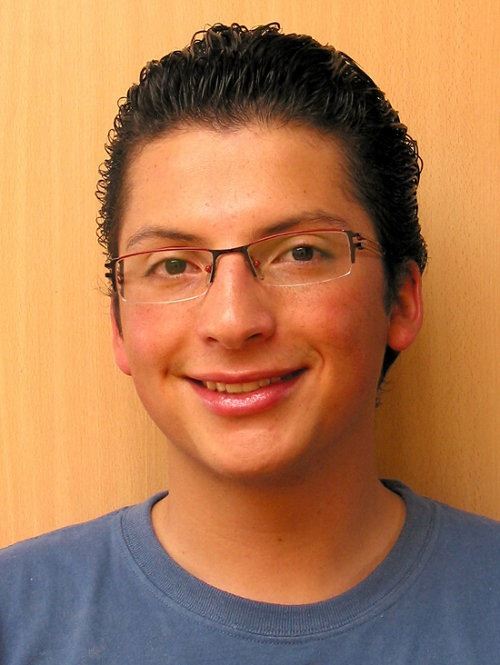
\includegraphics[width=3cm,bb=0 0 500 665]{./foto.jpg}}\\
    Cap. Rafael Ramos E2-254	& {\it mobile:} +(593-9) 643-9206 \\
    Casa \# 2			& {\it e-mail:}  onajera.fisica@epn.edu.ec\\
    Quito, Ecuador		& {\it www:} http://titan-c.github.com
  \end{tabular}\vspace{0.5cm}

\section{\sc Personal Information}
 \begin{tabular}{ll}
  {\it Family Name:} Nájera Ocampo & {\it Date of Birth:} 13 April 1988\\
  {\it Given Name:} Óscar Andrés   & {\it Gender:} Male\\
  {\it Nationality:} Ecuadorian    & %{\it Marital status:} Single
 \end{tabular}

\section{\sc Research Interests}
  Condensed Matter, Solid State Physics, Statistical Mechanics, Mathematical \& Theoretical Physics, Scientific Programming

\section{\sc Education}
  {\bf Escuela Politécnica Nacional}, Quito, Ecuador\\
  \vspace{-.1in}
  \begin{list1}
    \item[] Physics Diploma Student \hfill {\bf October 2006 - September 2012}\\
    \begin{list2}
    \vspace{-.1in}
      \item Thesis Topic:  ``Estimation, by computer simulation, of the exchange
	energy dispersion between polar nano-regions in $Pb_xBi_4Ti_{3+x}O_{12+3x}; x=\{2,3\}$
	relaxor ferroelectrics''
      \item Advisor: Dr. Luis Lascano
      \item Written in: Spanish
      \item Coursework grades: 8.2/10 | Written thesis: 9.8/10 | Oral examination: 10/10
    \end{list2}
  \end{list1}

  {\bf German School}, Quito, Ecuador\\
  \vspace{-.1in}
  \begin{list1}
    \item[] German Abitur \hfill {\bf May 2006}
    \item[] Ecuadorian High School Diploma \hfill {\bf June 2005}
  \end{list1}

\section{\sc Honors and Awards}
  Physics Olympiad $1^{st}$ place, Escuela Politécnica Nacional, Ecuador \hfill {\bf 2010}\\
  Bronze Medal for Academic performance, German School Quito, Ecuador \hfill {\bf 2005}\\
  PAD Preisträger, Kultusminister Konferenz, Germany \hfill {\bf 2003}

\section{\sc Academic Experience}
  {\bf Escuela Politécnica Nacional}, Quito, Ecuador
    \vspace{-.3cm}

    {\em Student} \hfill {\bf October 2006 - September 2012}\\
    Includes current research and coursework

    {\em Laboratory and teacher's Assistant} \hfill {\bf August 2011 - June 2012}\\
    Responsible of Experimental Physics laboratory in subjects
    like Newtonian Mechanics, Electromagnetism and Optics.
    Shared responsibility for lectures, homework assignments and grades.


  {\bf International Center for Theoretical Physics}, Trieste, Italy
    \vspace{-.3cm}

    {\em Invited Student} \hfill {\bf Feb 20 - Mar 2, 2012} \\
    Participation and presentation of research work at the {\em ``Advanced School on Scientific
    Software Development''} SMR 2330

\section{\sc Conference Presentations}
  Nájera, O.: ``Phase transitions in random interaction Ising-like models. Case study relaxor
  ferroelectrics'' {\bf In:} XVI ELAVIO, {\em Latin American School in Operations Research}, Feb 2012.

\section{\sc Other Publications}
  Nájera, O.: ``Estimation, by computer simulation, of the exchange energy dispersion between
  polar nano-regions in $Pb_xBi_4Ti_{3+x}O_{12+3x}; x=\{2,3\}$ relaxor ferroelectrics'', Thesis
  Preliminary Examination(Spanish). Department of Physics - Escuela Politécnica Nacional, April 2012.


\section{\sc Computer Skills}
  \begin{list2}
    \item Programming Languages:  C/C++, Python, Bash, Php, Matlab/Octave
    \item Content-description languages: \LaTeX, HTML, CSS
    \item Operating Systems:  Linux(Gentoo)
    \item Graphic design: Gimp, Inkscape, Blender
  \end{list2}

\section{\sc Languages}
  \begin{list2}
    \item Spanish: Native speaker
    \item English: Fluent speaker
    \item German: Fluent speaker
  \end{list2}
  
\section{\sc Personal Referees}
 \begin{list1}
  \item[] Dr. Luis Lascano
  \begin{list2}
   \item {\it e-mail:} luis.lascano@epn.edu.ec
   \item {\it Institution:} Escuela Politécnica Nacional
   \item Thesis supervisor \& teacher Solid State Physics
  \end{list2}
 \end{list1}
 \begin{list1}
  \item[] Dr. Leonardo Basile
  \begin{list2}
   \item {\it e-mail:} leonardo.basile@epn.edu.ec
   \item {\it Institution:} Escuela Politécnica Nacional
   \item Thesis examination committee \& teacher Statistical Physics
  \end{list2}
 \end{list1}


\section{\sc Outside Interests}
 \begin{list2}
  \item Ballroom Dancing
  \item Cycling
 \end{list2}

\end{resume}
\end{document}
